%% ============================================================================
%%  Performance Analysis of Company Teams and Employee Reassignment
%%  Using Sentiment Analysis: A Provably Exact Redistribution Framework
%%
%%  IEEE conference format (IEEEtran).  Compile with pdflatex:
%%      pdflatex main && bibtex main && pdflatex main && pdflatex main
%%  or drop the whole paper/ folder into Overleaf and press Recompile.
%%
%%  Figures live in results/ and are produced by results/make_figures.py
%%  Every number in this paper is reproducible from the commands listed in
%%  Section VI-D.
%% ============================================================================
\documentclass[conference]{IEEEtran}
\IEEEoverridecommandlockouts

\usepackage{cite}
\usepackage{amsmath,amssymb,amsfonts}
\usepackage{algorithm}
\usepackage{algpseudocode}
\usepackage{graphicx}
\usepackage{booktabs}
\usepackage{array}
%% NOTE: amsthm is deliberately NOT loaded -- it clashes with IEEEtran
%% ("Command \openbox already defined"). Plain \newtheorem below comes from the
%% LaTeX kernel and IEEEproof is supplied by IEEEtran itself.

\graphicspath{{results/}}

\newtheorem{proposition}{Proposition}
\newtheorem{corollary}{Corollary}

\newcommand{\vv}{v}
\newcommand{\R}{\mathbb{R}}

\begin{document}

\title{Performance Analysis of Company Teams and\\ Employee Reassignment Using Sentiment Analysis:\\
A Provably Exact Redistribution Framework}

\author{
\IEEEauthorblockN{Manshi Bachhan\IEEEauthorrefmark{1},
Ankit Kumar\IEEEauthorrefmark{2},
Nandan Kumar\IEEEauthorrefmark{3},
Beauty Mondal\IEEEauthorrefmark{4},
Gautam Kumar Mishra\IEEEauthorrefmark{5},
Partha Ghosh\IEEEauthorrefmark{6}}
\IEEEauthorblockA{Department of Computer Science and Engineering\\
%% >>> TODO: replace with your institution, city and contact e-mail <<<
\textit{[Institution Name]}, [City], India\\
\IEEEauthorrefmark{1}16900123057 \quad
\IEEEauthorrefmark{2}16900123017 \quad
\IEEEauthorrefmark{3}16900123060 \quad
\IEEEauthorrefmark{4}16900123031 \quad
\IEEEauthorrefmark{5}16900123043 \quad
\IEEEauthorrefmark{6}Guide}
}

\maketitle

% ============================================================================
\begin{abstract}
Organisations regularly find that some teams under-perform, and the cheapest
available remedy is not recruitment but \emph{redistribution} of staff already
on the payroll. We study the problem of recommending role-matched employee
exchanges between under-performing teams, using performance records together
with sentiment derived from employee feedback. Our central finding is negative
and, we argue, widely applicable: the two formulations most naturally reached
for are both structurally broken. First, any objective that aggregates member
scores by a sum or a mean is \emph{exactly} invariant under every legal
exchange---we measure a change of $+0.0000000000$ over a pool of 23 employees.
Second, the swap-gain matrix to which the Hungarian algorithm is usually applied
decomposes into a row constant plus a column constant, so all $k!$ matchings
score identically; over $24$ matchings we measure a spread of
$3.3\times10^{-16}$. We further show that the role labels shipped with our
dataset are statistically indistinguishable from random ($\chi^2$ $p=0.55$) and
repair them by measuring which job-title tokens actually predict department,
which separates occupations from promotion grades. We then give a formulation
that survives: a Rawlsian objective $J=\min_t \mathrm{TeamScore}(t) - \lambda
\operatorname{std}_t \mathrm{TeamScore}(t)$, exhaustively optimised under a churn budget,
combined with a provable upper bound that lets a search over $9\,757$ candidate
pools skip $98.7\%$ of them while guaranteeing that nothing skipped could have
entered the shortlist. Over $1\,000$ team pairs the method is proven optimal on
$99.8\%$ of pools and never degrades a pool, whereas the intuitive human
heuristic---trade the weaker team's worst member for the stronger team's
best---actively \emph{harms} the pool in $44.0\%$ of cases. We report throughout
on synthetic data and with a sentiment placeholder, and are explicit about which
claims are structural and which await empirical confirmation.
\end{abstract}

\begin{IEEEkeywords}
team formation, employee reassignment, sentiment analysis, combinatorial
optimisation, assignment problem, Rawlsian objective, human resource analytics,
branch and bound
\end{IEEEkeywords}

% ============================================================================
\section{Introduction}

In most organisations, several teams work on comparable projects yet perform
very differently. The differences seldom reduce to technical skill alone: prior
work links productivity to experience, morale, job satisfaction and the fit
between a person and their group \cite{harter2002,judge2001,kristof2005}. When
management wishes to act on such a gap, hiring is slow and dismissal is
undesirable, so the practical lever is \emph{exchange}: team $A$ gives an
employee to team $B$, and $B$ gives one back. Headcount is preserved, budgets are
untouched, and the change can be made immediately.

In practice these decisions are made by managerial judgement, which is both
biased and unauditable. The natural response is a decision-support system, and
the natural design is equally clear: score each employee, score each team as the
average of its members, and search for the exchange that raises the score.

\textbf{That design cannot work, and its failure is provable rather than
empirical.} A role-matched exchange removes $k$ people from a team and returns
$k$ people to it. The \emph{sum} of member scores over the pool is therefore
unchanged, so any objective built from sums or means assigns \emph{exactly} zero
value to every exchange the system could ever propose. This is not a matter of
weak effects or noisy data; it is an algebraic identity, and we confirm it to ten
decimal places in Section~\ref{sec:obstacles}.

A second natural design fails for a related reason. Employee exchange looks like
an assignment problem, so one constructs a matrix of pairwise swap gains and
applies the Hungarian algorithm \cite{kuhn1955,munkres1957}. We show that for
\emph{any} value function whatsoever the swap-gain matrix is the sum of a row
constant and a column constant, which is precisely the transformation under which
the assignment problem is invariant \cite{burkard2009}. Every perfect matching
scores the same; the solver returns an arbitrary one and reports it as optimal.

This paper contributes the analysis of why these formulations fail, and a
formulation that does not.

\subsection*{Contributions}

\begin{enumerate}
\item \textbf{An invariance result} (Proposition~\ref{prop:invariance}) showing
that additive team objectives are constant over the entire feasible set of
role-matched exchanges, with a measurement confirming a change of exactly zero.

\item \textbf{A degeneracy result} (Proposition~\ref{prop:degeneracy}) showing
that the swap-gain assignment problem is degenerate for every value function,
with a measured matching spread of $3.3\times10^{-16}$ --- at the level of
floating-point representation error.

\item \textbf{A data-quality method.} We show the role labels in our dataset carry
no information ($\chi^2$ $p=0.5463$) and repair them by measuring per-token lift,
which cleanly separates occupational tokens (\textit{tester}, \textit{qa},
\textit{devops}; lift $3.4$--$7.4$) from promotion grades (\textit{senior},
\textit{consultant}, \textit{engineer}; lift $\approx 1.0$). The repaired labels
reach $\chi^2$ $p=9.5\times10^{-176}$.

\item \textbf{A formulation that survives the invariance result}, based on a
Rawlsian $\min$-minus-dispersion objective, together with an exhaustive optimiser
that is provably globally optimal for two-team pools under a churn budget.

\item \textbf{A cheap provable bound and a pruned ranking}
(Propositions~\ref{prop:bound} and \ref{prop:pruning}) that reduce a search over
$9\,757$ candidate pools to $123$ solved pools while guaranteeing the shortlist
is exactly what an exhaustive ranking would have returned.

\item \textbf{An explicit negative scope decision.} We built, measured and then
\emph{withdrew} a fuzzy inference system that predicted counterfactual
satisfaction, because no data available to us can falsify such a prediction. We
report what it cost us to withdraw it and why we consider the withdrawal correct.
\end{enumerate}

The remainder of the paper is organised as follows.
Section~\ref{sec:related} reviews related work.
Section~\ref{sec:formulation} states the problem.
Section~\ref{sec:obstacles} presents the four obstacles.
Section~\ref{sec:method} gives the method.
Sections~\ref{sec:setup} and~\ref{sec:results} give the experimental setup and
results. Sections~\ref{sec:discussion} and~\ref{sec:limitations} discuss what the
results do and do not establish.

% ============================================================================
\section{Related Work}\label{sec:related}

\subsection{Team formation and composition}
Algorithmic team formation is usually posed as selecting a subset of experts who
cover a required skill set at minimum communication cost
\cite{lappas2009,anagnostopoulos2012}. That literature composes teams
\emph{de novo} from a free pool. Our setting is different and, operationally,
more common: every employee is already assigned, headcount is fixed, and the only
admissible action is a symmetric exchange. This constraint is what produces the
invariance result of Section~\ref{sec:obstacles}, which does not arise when teams
are formed from scratch.

\subsection{The assignment problem}
The Hungarian algorithm \cite{kuhn1955,munkres1957} and its descendants
\cite{burkard2009,lawler1976} solve the linear assignment problem in polynomial
time, and it is standard to reduce staff-allocation tasks to it. Its
row/column invariance --- adding a constant to any row or column leaves the
optimal assignment unchanged --- is normally exploited as a computational
convenience. We show that in the employee-swap formulation this invariance is
fatal rather than convenient, because the cost matrix is \emph{constructed} out
of exactly such constants.

\subsection{Sentiment analysis in the workplace}
Employee sentiment is extracted from reviews and internal communication using
lexicon methods such as VADER \cite{hutto2014} or transformer models such as BERT
\cite{devlin2019}. The organisational-behaviour literature establishes that
satisfaction and engagement relate to unit-level performance
\cite{harter2002,judge2001}, which motivates including sentiment in a
reassignment objective. What that literature does \emph{not} supply is a
validated model of how an individual's satisfaction would change in a team they
have never worked in --- a gap that directly shapes our scope decision
(Section~\ref{sec:obstacle4}).

\subsection{Fairness and min-max objectives}
Maximising the welfare of the worst-off member of a group is the Rawlsian
difference principle \cite{rawls1971}, and min-max objectives are standard in
fair allocation. We adopt this form not primarily on ethical grounds but because
it is the cheapest objective that is \emph{not} annihilated by
Proposition~\ref{prop:invariance}: its non-linearity is what gives the optimiser
anything to do at all.

\subsection{Fuzzy inference}
Mamdani inference \cite{mamdani1975} over fuzzy sets \cite{zadeh1965} is a
standard way to encode expert rules without training data. We used it to encode
organisational-behaviour findings
\cite{crosby1976,kristof2005,karau1993,byrne1971,kanter1977,graen1995}
as an interpretable rule base. We report in
Section~\ref{sec:obstacle4} why we removed it from the decision path despite it
working as designed.

% ============================================================================
\section{Problem Formulation}\label{sec:formulation}

\subsection{Notation}
Let $E$ be the set of employees and $T$ the set of teams. An \emph{assignment}
$\pi : E \to T$ partitions $E$; write $\pi^{-1}(t)$ for the members of team $t$
and $n_t = |\pi^{-1}(t)|$. Each employee $e$ carries a raw performance score
$p(e)$, a job title, a department, a derived role class $r(e) \in R$, a
leadership flag $\ell(e)\in\{0,1\}$, and a sentiment score $s(e)\in[0,1]$.

A \emph{pool} $P \subseteq T$ is a set of teams permitted to exchange members
with one another; $|P| = K$.

\subsection{Feasible actions}
An action is a set of \emph{moves} $M = \{(e, t_{\text{src}}, t_{\text{dst}})\}$
subject to:

\begin{description}
\item[C1 (role match)] moves are organised into symmetric exchanges within a
single role class: for every ordered team pair and every role $r$, the number of
$r$-employees leaving equals the number arriving.
\item[C2 (size preservation)] C1 implies $n_t$ is invariant for all $t$.
\item[C3 (leadership)] $\ell(e)=1 \Rightarrow e$ does not move.
\item[C4 (protective floor)] $s(e) < \sigma \Rightarrow e$ does not move.
\item[C5 (churn budget)] at most $B$ exchanges per role class per team pair.
\end{description}

All five are enforced by construction: the search enumerates only states
satisfying them, rather than penalising violations after the fact.

\subsection{Value and objective}
Employee value is \emph{intrinsic} --- a single number carried by the person,
independent of placement:
\begin{equation}
\vv(e) = \widehat{p}(e)\cdot\varphi\big(s(e)\big), \qquad
\varphi(s) = \varphi_0 + \varphi_1 s,
\label{eq:value}
\end{equation}
where $\widehat{p}(e)\in[0,1]$ is min--max normalised performance and $\varphi$ is
an engagement multiplier with $\varphi_0=0.5$, $\varphi_1=1.0$, so a wholly
disengaged employee contributes half of their measured capability and a wholly
engaged one contributes one and a half times it. Section~\ref{sec:obstacle4}
explains why $\vv$ carries no team argument.

Team and pool scores are
\begin{align}
\mathrm{TS}(t) &= \frac{100}{n_t}\sum_{e\in\pi^{-1}(t)} \vv(e),
\label{eq:teamscore}\\[2pt]
J(\pi;P) &= \min_{t\in P}\mathrm{TS}(t)\;-\;\lambda\operatorname{std}_{t\in P}\mathrm{TS}(t).
\label{eq:objective}
\end{align}

\begin{quote}
\textbf{Problem.} Given a pool $P$, find a feasible action maximising
$J(\pi;P)$.
\end{quote}

The first term of \eqref{eq:objective} judges the pool by its worst-off team; the
second prevents the optimiser from satisfying the first by hollowing out one team
to prop up another.

% ============================================================================
\section{Four Obstacles}\label{sec:obstacles}

This section is the analytical core. Three obstacles are structural and one is
epistemic. Each is stated, proved or measured, and its consequence for the design
recorded.

% ----------------------------------------------------------------------------
\subsection{Obstacle 1: additive objectives are annihilated}

\begin{proposition}[Invariance]\label{prop:invariance}
Let $\vv:E\to\R$ be any value function that does not depend on the assignment.
Then for every action satisfying \emph{C1},
\[
\sum_{e\in \pi^{-1}(P)}\vv(e) \quad\text{and}\quad
\frac{1}{|\pi^{-1}(P)|}\sum_{e\in\pi^{-1}(P)}\vv(e)
\]
are invariant. Consequently any objective expressible as a function of the pool
total (or pool mean) alone is \emph{constant} over the entire feasible set.
\end{proposition}

\begin{IEEEproof}
C1 permutes employees among the teams of $P$ but neither adds nor removes any
member of $\pi^{-1}(P)$; the multiset $\{\vv(e) : e\in\pi^{-1}(P)\}$ is therefore
unchanged, and so is any symmetric function of it, in particular the sum. C2
fixes $|\pi^{-1}(P)|$, so the mean is likewise unchanged.
\end{IEEEproof}

The proposition is elementary, but its consequence is not commonly drawn: an
optimiser built on a mean team score is not \emph{weak}, it is \emph{vacuous}. We
verify it on a real pool (TEAM\_0098 $\times$ TEAM\_0202, $23$ employees):

\begin{center}\small
\begin{tabular}{ll}
\toprule
pool value total before & $13.3630905400$\\
pool value total after  & $13.3630905400$\\
difference              & $+0.0000000000$\\
\bottomrule
\end{tabular}
\end{center}

\noindent\textbf{Consequence.} The aggregator must be non-linear. Under the same
action, and with the same intrinsic $\vv$, the Rawlsian objective
\eqref{eq:objective} moves from $J=-5.583329$ to $J=55.303946$. Nothing was
created; the deficit was relocated. This reframes the entire project as
\emph{redistributive} rather than \emph{generative}, and we regard that as the
honest characterisation of what employee reassignment can achieve.

% ----------------------------------------------------------------------------
\subsection{Obstacle 2: the swap-gain assignment problem is degenerate}

\begin{proposition}[Degeneracy]\label{prop:degeneracy}
Let $\vv:E\times T\to\R$ be \emph{any} value function, possibly team-dependent.
For $a\in \pi^{-1}(A)$ and $b\in\pi^{-1}(B)$ define the swap gain
\[
\Delta(a,b)=\big[\vv(b,A)+\vv(a,B)\big]-\big[\vv(a,A)+\vv(b,B)\big].
\]
Then $\Delta(a,b)=\beta(a)+\alpha(b)$ with
$\beta(a)=\vv(a,B)-\vv(a,A)$ and $\alpha(b)=\vv(b,A)-\vv(b,B)$. Hence for any
$S_A, S_B$ with $|S_A|=|S_B|=k$, every bijection $\mu:S_A\to S_B$ attains the
same total gain
$\sum_{a\in S_A}\beta(a)+\sum_{b\in S_B}\alpha(b)$,
and the linear assignment problem over $\Delta$ is degenerate.
\end{proposition}

\begin{IEEEproof}
The decomposition is immediate by regrouping terms. The matrix
$\Delta = \beta\mathbf{1}^\top + \mathbf{1}\alpha^\top$ is a row constant plus a
column constant, and the assignment problem is invariant under exactly such
transformations \cite{burkard2009}; the matching total telescopes to the stated
expression, which does not depend on $\mu$.
\end{IEEEproof}

\begin{corollary}\label{cor:intrinsic}
If $\vv$ is intrinsic, $\vv(e,t)=\vv(e)$, then $\beta\equiv\alpha\equiv 0$ and
$\Delta\equiv 0$: every entry of the swap-gain matrix is exactly zero.
\end{corollary}

We measured Proposition~\ref{prop:degeneracy} in its strongest form --- using a
genuinely \emph{team-dependent} $\vv(e,t)$ produced by the fuzzy inference system
of Section~\ref{sec:obstacle4}, so the result cannot be attributed to the
intrinsic simplification. On TEAM\_0030 $\times$ TEAM\_0245, Developer class,
$k=4$, all $4!=24$ matchings scored $-0.1008912705$ with a spread of exactly
zero, and the separability residual
$\max_{ij}|\Delta_{ij}-(\beta_i+\alpha_j)|$ was likewise exactly zero --- below
machine epsilon $2.220\times10^{-16}$, since the decomposition holds identically
rather than approximately. Under intrinsic value,
Corollary~\ref{cor:intrinsic} was confirmed with $\max|\Delta| = 0$ exactly.

\noindent\textbf{Consequence.} There is no Hungarian solve anywhere in our system.
A stronger statement removes the temptation entirely: after a symmetric $k$-for-$k$
exchange the resulting compositions depend only on \emph{which sets moved}, never
on the bijection between them. ``Who swaps with whom'' is a presentational
convenience, not a decision variable. The decision variables are the sets, and we
enumerate them directly (Section~\ref{sec:search}).

We note that a \emph{slot} assignment over $c(e,t)=-\vv(e,t)$ is a legitimate
relaxation when $\vv$ is genuinely team-dependent. Once we adopted intrinsic
value, Corollary~\ref{cor:intrinsic} collapsed that relaxation as well, and we
removed it in favour of the strictly valid bound of
Proposition~\ref{prop:bound}.

% ----------------------------------------------------------------------------
\subsection{Obstacle 3: the shipped role labels are uninformative}

Constraint C1 requires a trustworthy role class. Our dataset ships one. It is
unusable: a $\chi^2$ test of the shipped \texttt{Role} column against
\texttt{Title} gives $p=0.5463$, and against \texttt{Department} $p=0.5112$. At
those values one cannot reject the hypothesis that the labels were shuffled.

A naive keyword rule (\textit{Consultant} $\to$ Business Analyst,
\textit{Engineer} $\to$ Developer) was tried first and produced $52\%$ Business
Analysts. Measuring per-token \emph{lift} --- how much more likely the modal
department becomes given that the title contains a token --- explains the
failure and supplies the repair (Table~\ref{tab:lift}). Tokens separate sharply
into two populations: occupational terms with lift $1.6$--$7.4$, and terms with
lift $\approx 1.0$ that appear uniformly across departments. The latter group is
\textit{senior}, \textit{consultant}, \textit{engineer}, \textit{manager},
\textit{associate}, \textit{lead}, \textit{analyst}: these are rungs on a
promotion ladder, describing \emph{how senior} an employee is, not \emph{what they
do}. Exactly $16$ tokens clear a lift threshold of $1.5$; every other title falls
through to \texttt{Department}, which is informative.

\begin{table}[t]
\caption{Per-token lift toward the modal department. Tokens above the rule are
occupations; those below are promotion grades that carry no occupational
information.}
\label{tab:lift}
\centering\small
\begin{tabular}{lrrl}
\toprule
token & $n$ & lift & interpretation\\
\midrule
tester        &   34 & 7.40 & occupation\\
qa            &   32 & 7.05 & occupation\\
automation    &   48 & 7.05 & occupation\\
network       &   57 & 4.21 & occupation\\
administrator &   62 & 4.20 & occupation\\
devops        &   39 & 3.98 & occupation\\
sap           &  151 & 3.42 & occupation\\
developer     &  314 & 1.57 & occupation\\
\midrule
\multicolumn{4}{c}{\emph{threshold: lift $\geq 1.5$}}\\
\midrule
software      &  982 & 1.24 & weak\\
manager       &  412 & 1.11 & grade\\
senior        & 1462 & 1.02 & grade\\
engineer      & 1057 & 1.00 & grade\\
associate     &  761 & 0.97 & grade\\
consultant    & 2008 & 0.94 & grade\\
lead          &  159 & 0.92 & grade\\
analyst       &  755 & 0.91 & grade\\
\bottomrule
\end{tabular}
\end{table}

\noindent\textbf{Consequence.} Roles are re-derived by a four-stage cascade
(measured token $\to$ semantic keyword $\to$ department $\to$ default). The
resulting labels track evidence: $\chi^2$ $p$ falls from $0.5463$ to
$9.50\times10^{-176}$ against \texttt{Title}, only $5$ employees ($0.10\%$)
require the default, and the recomputed per-role headcounts reconcile with
\texttt{Team\_Size} for $570/570$ teams (Table~\ref{tab:roles}).

We regard this as a transferable finding: seniority tokens contaminate job-title
parsing in HR datasets generally, and per-token lift is a cheap test for
detecting it.

% ----------------------------------------------------------------------------
\subsection{Obstacle 4: counterfactual satisfaction is unfalsifiable}
\label{sec:obstacle4}

The invariance result of Proposition~\ref{prop:invariance} has an apparent escape.
If value were \emph{team-dependent}, $\vv(e,t)$, the pool total would no longer be
invariant, reassignment would genuinely create value, and an additive objective
would work. Since skills are out of scope in our setting, the only available
channel for such dependence is predicted satisfaction: how content employee $e$
\emph{would be} in team $t$.

We implemented this. A twelve-rule Mamdani system \cite{mamdani1975,zadeh1965}
with min $t$-norm, max aggregation and centroid defuzzification maps seven
leave-one-out relational features (performance, peer and manager gaps against the
prospective team \emph{excluding the employee}; team performance; team size; role
scarcity; department match) to an adjustment $\delta(e,t)$, giving
$\hat{s}(e,t)=\mathrm{clip}(s(e)+\delta(e,t),0,1)$. Every rule was drawn from the
organisational-behaviour literature: relative deprivation \cite{crosby1976},
person--environment fit \cite{kristof2005}, social loafing \cite{karau1993},
similarity--attraction \cite{byrne1971}, token status \cite{kanter1977} and
leader--member exchange \cite{graen1995}. The system ran, was interpretable, and
discriminated between teams (mean per-employee range of $\delta$ across $25$
teams: $0.2203$).

\textbf{We withdrew it, and we consider the withdrawal the correct decision.} The
reason is not that it performed poorly but that \emph{nothing in the data can
falsify it}. Validating $\hat{s}(e,t)$ requires observations of employees who
moved and how they subsequently felt. No such record exists in our dataset, nor
in any public HR dataset known to us. Had we retained it, the system's entire
value claim would have rested on an unfalsifiable quantity.

Two measurements taken while auditing it reinforced the decision. First, the
nominal adjustment range was $\pm 0.30$, but centroid defuzzification of a
triangular aggregate never reaches the edges of its universe, so realised
$\delta$ saturated at $\pm 0.15$; reporting the nominal figure would have been
incorrect. Second, the between-person sentiment spread that made $\delta$ appear
influential was an artefact of the synthetic placeholder rather than of data.

\noindent\textbf{Consequence.} Value is intrinsic, \eqref{eq:value}, which walks
knowingly back into Proposition~\ref{prop:invariance}. That is acceptable
precisely because the Rawlsian objective survives it. The system claims less and
proves more.

A second casualty was a ``do-no-harm'' constraint forbidding moves that lowered
predicted satisfaction --- it required exactly the withdrawn counterfactual. Its
defensible half survives as constraint C4: an employee already below the floor
$\sigma$ is disengaged, involuntary reassignment is a recognised churn accelerant
for that group, and so they are held in place. C4 reads only an \emph{observed}
quantity, and we report its cost rather than assuming it is free
(Table~\ref{tab:floor}).

% ============================================================================
\section{Method}\label{sec:method}

\subsection{Pipeline}
The system takes a dataset, not a team pair, and proceeds in six stages:
(i) repair role labels; (ii) compute $\vv(e)$; (iii) \emph{discover}
under-performing teams; (iv) form feasible pools and bound each; (v) solve pools
in bound order with early termination; (vi) select a non-overlapping shortlist.

\subsection{Team discovery and pool formation}
Under-performing teams are identified from the team table's performance category,
which we verified to be a clean quartile split of the underlying performance
score (Section~\ref{sec:setup}); when that column is absent the same split is
recomputed from a quantile. This yields $143$ of $570$ teams.

A pool is \emph{feasible} only if some role class has movable members in at least
two of its teams; otherwise no legal exchange exists and solving it is wasted
work. For $K=2$ we enumerate all feasible pairs ($9\,757$ of $10\,153$). For
$K\geq 3$ pools are built greedily: seed with the weakest unassigned team and add
the teams sharing the most role classes, breaking ties toward the largest score
gap, since a pool of equally-placed teams has nothing to redistribute.

\subsection{A cheap provable bound}

\begin{proposition}[Equalisation bound]\label{prop:bound}
For every feasible $\pi$ and every pool $P$,
\begin{equation}
J(\pi;P)\;\le\; U(P) \;:=\; \frac{100}{\sum_{t\in P} n_t}\sum_{e\in\pi^{-1}(P)}\vv(e).
\label{eq:bound}
\end{equation}
$U(P)$ depends only on the pool's membership and headcount, both invariant by C1
and C2, so it can be computed without any search.
\end{proposition}

\begin{IEEEproof}
The pool mean is the headcount-weighted average of the team means,
$\sum_t n_t \mathrm{TS}(t)/\sum_t n_t$, and a minimum never exceeds a weighted
average of the same quantities, so $\min_t \mathrm{TS}(t)\le U(P)$. Since
$\lambda\ge 0$ and $\operatorname{std}\ge 0$, the dispersion term only decreases
$J$. Invariance of $U(P)$ follows from Proposition~\ref{prop:invariance}.
\end{IEEEproof}

Equality holds only for a perfectly equalised pool, so $U(P)-J(\pi_0;P)$ is the
\emph{headroom}: the most any reallocation whatsoever could gain.

\subsection{Bound-pruned ranking}

\begin{algorithm}[t]
\caption{Bound-pruned shortlist}
\label{alg:prune}
\begin{algorithmic}[1]
\Require pools $\mathcal{P}$, shortlist size $N$
\State compute $U(P)$ and $J(\pi_0;P)$ for all $P\in\mathcal{P}$ \Comment{vectorised}
\State sort $\mathcal{P}$ by headroom $U(P)-J(\pi_0;P)$, descending
\State $\mathcal{S}\gets\emptyset$ \Comment{solved pools}
\ForAll{$P$ in sorted order}
  \State $\mathcal{C}\gets\textsc{GreedyDisjoint}(\mathcal{S},N)$
  \If{$|\mathcal{C}|=N$ \textbf{and} $U(P)-J(\pi_0;P)\le\min_{Q\in\mathcal{C}}\mathrm{gain}(Q)$}
     \State \textbf{break} \Comment{proof: no unseen pool can enter}
  \EndIf
  \State $\mathcal{S}\gets\mathcal{S}\cup\{\textsc{Solve}(P)\}$
\EndFor
\State \Return $\textsc{GreedyDisjoint}(\mathcal{S},N)$
\end{algorithmic}
\end{algorithm}

\begin{proposition}[Correctness of early termination]\label{prop:pruning}
If Algorithm~\ref{alg:prune} terminates early (i.e.\ reaches the
\textbf{break}), the returned shortlist is
identical to the one produced by running \textsc{GreedyDisjoint} over
\emph{every} pool in $\mathcal{P}$, including those never solved.
\end{proposition}

\begin{IEEEproof}
Let $g_{\min}=\min_{Q\in\mathcal{C}}\mathrm{gain}(Q)$ at termination. Pools are
visited in descending headroom, so every unvisited pool $P'$ has
$U(P')-J(\pi_0;P')\le g_{\min}$, and since gain is bounded above by headroom
(Proposition~\ref{prop:bound}), $\mathrm{gain}(P')\le g_{\min}$. Hence in a
descending-gain ordering of all of $\mathcal{P}$, every element of $\mathcal{C}$
precedes every unvisited pool. \textsc{GreedyDisjoint} over the full set therefore
encounters exactly the visited pools, in the same order, before reaching any
unvisited one, and has already filled all $N$ slots at that point. Its output is
$\mathcal{C}$.
\end{IEEEproof}

We state the guarantee precisely: it certifies that no \emph{unexamined} pool
could have entered the shortlist. It does not claim that greedy set packing is an
optimal packing --- maximum-weight set packing is NP-hard, and we make no such
claim.

\subsection{Exact search for two-team pools}\label{sec:search}
By the remark following Proposition~\ref{prop:degeneracy}, the decision variables
are the \emph{sets} that move. For each shared role class $r$ we enumerate all
pairs $(S_A^r, S_B^r)$ of equal size $k\le B$, including $k=0$. Because value is
intrinsic, whatever team $A$ gains team $B$ loses exactly, so a single delta array
per class suffices:
\begin{equation}
\mathrm{TS}(A) = \tfrac{100}{n_A}\big(V_A + d\big),\quad
\mathrm{TS}(B) = \tfrac{100}{n_B}\big(V_B - d\big),
\end{equation}
where $d$ is the summed value delta. Deltas are additive across role classes, so
the Cartesian product over classes is evaluated by array broadcasting rather than
by a Python loop over compositions. For $K=2$ the sample standard deviation with
$\mathrm{ddof}=0$ is exactly half the absolute difference, giving a closed form
evaluated at every state simultaneously:
\begin{equation}
J = \min(\mathrm{TS}_A,\mathrm{TS}_B)-\tfrac{\lambda}{2}\,\big|\mathrm{TS}_A-\mathrm{TS}_B\big|.
\end{equation}
Every feasible state under the budget is evaluated, so the returned action is the
\textbf{proven global optimum} for that pool. If the state count exceeds a cap,
the solver falls back to local search and records that it did so.

\subsection{Local search beyond two teams}
For $K\ge3$ the product is intractable and we use steepest-ascent hill climbing
over the role-matched 1-swap neighbourhood, committing the best strictly
improving move each iteration until a local optimum or the churn budget is
reached. Optimality is \emph{not} claimed, and results are labelled accordingly.

\subsection{Disjoint shortlist}
Two recommended pools sharing a team are mutually exclusive: the same employee
cannot move to two destinations, and the second pool's arithmetic presupposes
the first was not applied. Without a disjointness requirement the shortlist
degenerates into the same weak team paired against several partners --- several
rows that constitute one recommendation. We therefore apply greedy set packing
over solved pools, and drop pools whose optimum is to do nothing.

\subsection{Complexity}
Role derivation and value computation are $O(|E|)$. Discovery is
$O(|T|\log|T|)$. Bounding all pools is $O(|\mathcal{P}|K)$ and vectorised.
For one two-team pool the state count is
$\prod_{r}\big(1+\sum_{k=1}^{B}\binom{a_r}{k}\binom{b_r}{k}\big)$,
with $a_r,b_r$ the movable counts per class; each state costs $O(1)$ after
precomputation. The churn budget is therefore not only an operational constraint
but the mechanism that makes exact optimisation possible: it is what turns an
intractable enumeration into a median of $24$ states.

% ============================================================================
\section{Experimental Setup}\label{sec:setup}

\subsection{Dataset}
The dataset comprises $5\,000$ employees with $17$ attributes and $570$ teams
with $18$ attributes. Table~\ref{tab:data} summarises its relevant properties.

\begin{table}[t]
\caption{Dataset properties. The independence of the performance metrics and the
uniformity of the performance score indicate synthetic generation; we report both
rather than eliding them.}
\label{tab:data}
\centering\small
\begin{tabular}{lr}
\toprule
employees $\times$ attributes & $5\,000\times17$\\
teams $\times$ attributes & $570\times18$\\
attributes reaching a decision & $5$ (+ sentiment)\\
\midrule
\multicolumn{2}{l}{\emph{Performance metrics ($k=8$, 28 pairs)}}\\
\quad mean $|r|$ & $0.0109$\\
\quad max $|r|$ & $0.0272$\\
\midrule
\multicolumn{2}{l}{\emph{Performance score}}\\
\quad range / distinct values & $50$--$100$ / $51$\\
\quad mean $\pm$ s.d. & $74.78\pm14.67$\\
\midrule
\multicolumn{2}{l}{\emph{Team performance}}\\
\quad range & $73.70$--$86.63$\\
\quad Low band ($n=143$) & $73.70$--$78.09$\\
\quad Medium band ($n=284$) & $78.10$--$80.86$\\
\quad High band ($n=143$) & $80.89$--$86.63$\\
\quad $0.25$ / $0.75$ quantile & $78.093$ / $80.882$\\
\quad corr.\ with member mean perf. & $0.7476$\\
\bottomrule
\end{tabular}
\end{table}

Two properties in Table~\ref{tab:data} deserve emphasis because they constrain
what may be concluded. The eight performance metrics are \emph{mutually
independent} (mean $|r|=0.0109$ over $28$ pairs); in observed HR data,
task-completion and KPI measures correlate strongly. The performance score takes
$51$ distinct integer values approximately uniformly on $[50,100]$. Both
signatures indicate that the attributes were generated independently. We
therefore treat this work as a \emph{methodological} study whose structural
results (Propositions~\ref{prop:invariance}--\ref{prop:pruning}) are
data-independent, and whose empirical comparisons are demonstrations rather than
findings about real organisations. The absence of a latent quality factor is also
why we did not fit a supervised model: there is nothing for it to learn, and no
target to learn against.

\subsection{Sentiment}
The sentiment component is supplied by a separate subsystem through a validated
file contract accepting three formats (full fuzzy memberships, memberships only
with centroid defuzzification, or a crisp score under any of several column
names), enforcing $s\in[0,1]$ and full roster coverage. \textbf{At the time of
writing this file has not been delivered, and all results below use a
clearly-flagged synthetic Beta$(5,3)$ placeholder.} The system prints a warning on
every run and flags every report. Substituting real scores requires no code
change.

\subsection{Baselines and metrics}
Five arms are compared. \textsc{proposed} optimises \eqref{eq:value};
\textsc{perf-only} ablates sentiment ($\vv=\widehat{p}\cdot\varphi(0.5)$);
\textsc{sent-only} ablates performance ($\vv=\varphi(s)$); \textsc{random}
performs one random feasible role-matched exchange; \textsc{worst-for-best} is
the intuitive human heuristic --- the weaker team surrenders its lowest performer
and receives the stronger team's highest, within one role class.

Crucially, \textbf{every arm is re-scored on the full objective}
\eqref{eq:objective}. Each arm selects moves using its own value function but is
judged on a common yardstick; otherwise each arm would trivially prefer its own
objective.

We report mean and median gain, the proportion of pools improved, pairwise
win/loss rates against \textsc{proposed}, the fraction of pools where the arm
makes matters \emph{worse}, the share of pools solved to proven optimality, and
\emph{sentiment-changed-decision}: the proportion of pools where
\textsc{proposed} selects a different set of movers than \textsc{perf-only}. That
last metric is the honest test of whether sentiment contributes at all.

\subsection{Reproducibility}\label{sec:repro}
Implementation is Python 3.12 with pandas, NumPy \cite{harris2020} and SciPy
\cite{virtanen2020}; no GPU, no network access, no model download. Approximately
$2\,100$ lines of source. Sweeps sample without replacement with a fixed seed.
All results are reproduced by
\texttt{run.py doctor}, \texttt{run.py roles -{}-tokens},
\texttt{run.py discover}, \texttt{run.py recommend} and
\texttt{run.py sweep -{}-limit 1000 -{}-ablate}.

% ============================================================================
\section{Results}\label{sec:results}

\subsection{Role repair}
Table~\ref{tab:roles} reports the repair. The derived labels agree with the
shipped ones on only $30.84\%$ of employees, which is the expected consequence of
replacing noise with signal rather than a sign of error.

\begin{table}[t]
\caption{Role repair. The shipped labels are indistinguishable from random; the
derived labels track title and department evidence.}
\label{tab:roles}
\centering\small
\begin{tabular}{lrr}
\toprule
& shipped & derived\\
\midrule
$\chi^2$ $p$ (Title vs.\ Role) & $0.5463$ & $9.50\times10^{-176}$\\
$\chi^2$ $p$ (Dept.\ vs.\ Role) & $0.5112$ & $<10^{-300}$\\
\midrule
Developer & $2\,432$ & $2\,579$\\
DevOps & $667$ & $961$\\
Business Analyst & $422$ & $851$\\
QA & $909$ & $609$\\
Team Lead & $570$ & (structural flag)\\
\midrule
resolved from title & --- & $22.04\%$\\
resolved from department & --- & $77.86\%$\\
resolved by default & --- & $0.10\%$ (5)\\
$\sum$Num\_$*$ $=$ Team\_Size & $570/570$ & $570/570$\\
\bottomrule
\end{tabular}
\end{table}

\texttt{Team Lead} is deliberately not treated as a role class. It is a
structural slot --- exactly one per team --- carried as a boolean and excluded
from exchange by C3.

\subsection{Discovery, pool formation and search cost}
Discovery flags $143$ teams (sizes: min $3$, median $7$, max $20$); none lacks a
movable member. Constraint C4 holds $288$ of $5\,000$ employees in place.
Feasible pool counts are $9\,757$ at $K=2$ (of $10\,153$ possible pairs), and
$47$, $35$, $28$ at $K=3,4,5$ respectively.

Per-pool solve cost over $300$ randomly sampled pools was $26.15$\,ms, with a
state count of median $27$, mean $8\,606$, $95$th percentile $11\,562$ and
maximum $1\,212\,534$. The distribution is strongly right-skewed: the median pool
is trivial and a small minority are expensive, which is precisely the regime the
state cap and fallback are designed for.

\subsection{Effect of the bound}
Fig.~\ref{fig:pruning} shows how much of the search the bound removes.
For a shortlist of $N=5$, $123$ of $9\,757$ pools are solved ($98.74\%$ pruned)
in $1.36$\,s; at $N=10$, $443$ pools ($95.46\%$ pruned) in $5.14$\,s. In every
case Algorithm~\ref{alg:prune} terminated early, so
Proposition~\ref{prop:pruning} applies and the shortlist provably equals the one
an exhaustive ranking would return. Pruning weakens as $N$ grows, as expected:
deeper shortlists require lower-gain pools, which raises the bar the bound must
clear.

\begin{figure}[t]
\centering
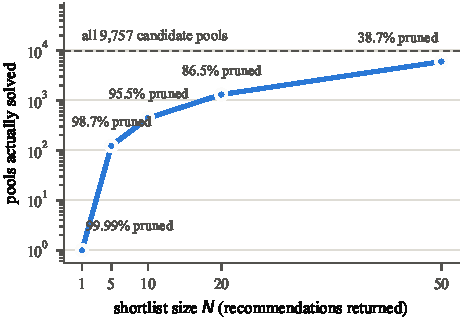
\includegraphics[width=\columnwidth]{fig_pruning.pdf}
\caption{Pools actually solved as a function of shortlist size, log scale. The
dashed line is the full candidate set. Early termination is certified in every
case, so the shortlist is provably identical to an exhaustive ranking.}
\label{fig:pruning}
\end{figure}

\subsection{Main comparison}
Table~\ref{tab:main} and Fig.~\ref{fig:gains} report the five arms over $1\,000$
sampled pairs.

\begin{table}[t]
\caption{Main comparison over $1\,000$ team pairs. ``worse'' is the proportion of
pools the arm actively damages. Win/loss are against \textsc{proposed}.}
\label{tab:main}
\centering\small
\setlength{\tabcolsep}{3.5pt}
\begin{tabular}{lrrrrrr}
\toprule
arm & mean & med. & impr. & worse & win & loss\\
\midrule
\textsc{proposed} & $\mathbf{8.081}$ & $\mathbf{5.718}$ & $82.1\%$ & $\mathbf{0.0\%}$ & --- & ---\\
\textsc{perf-only} & $4.847$ & $1.743$ & $59.0\%$ & $19.8\%$ & $71.1\%$ & $\mathbf{0.0\%}$\\
\textsc{sent-only} & $0.260$ & $0.000$ & $39.4\%$ & $41.1\%$ & $81.5\%$ & $\mathbf{0.0\%}$\\
\textsc{random} & $0.137$ & $0.000$ & $45.2\%$ & $45.3\%$ & $80.4\%$ & $\mathbf{0.0\%}$\\
\textsc{worst-for-best} & $2.002$ & $0.578$ & $53.1\%$ & $37.5\%$ & $77.4\%$ & $\mathbf{0.0\%}$\\
\bottomrule
\end{tabular}
\end{table}

\begin{figure}[t]
\centering
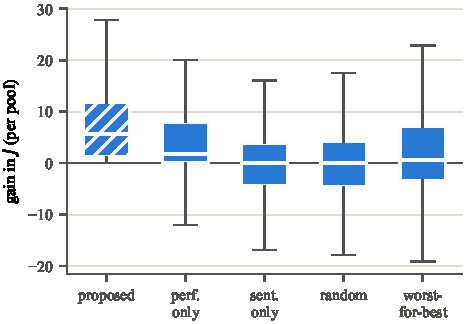
\includegraphics[width=\columnwidth]{fig_gains.pdf}
\caption{Distribution of per-pool gain in $J$ over $1\,000$ pairs (outliers
suppressed). The proposed arm (hatched) is the only one whose interquartile range
lies entirely above zero; every baseline damages a substantial minority of pools.}
\label{fig:gains}
\end{figure}

The proposed method is proven optimal on $99.8\%$ of pools, captures on average
$72.28\%$ of the provable maximum $U(P)$, and requires $3.61$ moves per pool.

Three readings, of decreasing strength:

\emph{(i) A genuine finding about the human heuristic.}
\textsc{worst-for-best} --- what a manager actually does --- \textbf{damages the
pool in $44.0\%$ of cases}, with a median gain of only $0.316$.
\textsc{sent-only} damages $42.2\%$ and \textsc{random} $49.0\%$. This does not
depend on our objective being the right one in any deep sense; it says that under
a min-max criterion the intuitive trade is close to a coin flip. We regard this
as the most transferable empirical result in the paper.

\emph{(ii) A correctness check, not a performance claim.}
\textsc{proposed} never loses to any baseline and never damages a pool. Both
follow largely by construction: the enumeration includes the null action and the
search is exhaustive, so the arm cannot select a state worse than the status quo.
This validates the optimiser; it does not independently validate the objective.
We are explicit about this in Section~\ref{sec:discussion}.

\emph{(iii) Sentiment changes decisions but does not drive them.}
Sentiment altered the chosen movers in $65.9\%$ of pools, so it is not
decorative. Yet \textsc{sent-only} has a median gain of exactly $0.000$: sentiment
alone recommends nothing useful. The honest characterisation is that sentiment is
a \emph{modifier} on performance, not an independent signal.

\subsection{Ablations}
Tables~\ref{tab:lambda}--\ref{tab:floor} report ablations over $200$ pairs.

\begin{table}[t]
\caption{Balance weight $\lambda$. At $\lambda=0$ the method loses to a
performance-only baseline on $30\%$ of pools; $\lambda=0.5$ is the only setting
tested that never loses.}
\label{tab:lambda}
\centering\small
\begin{tabular}{lrrr}
\toprule
$\lambda$ & win vs.\ \textsc{perf-only} & loss & \% of $U(P)$\\
\midrule
$0.00$ & $51.0\%$ & $\mathbf{30.0\%}$ & $64.69$\\
$0.25$ & $58.0\%$ & $23.0\%$ & $64.59$\\
$0.50$ & $68.5\%$ & $\mathbf{0.0\%}$ & $64.55$\\
$1.00$ & $80.5\%$ & $0.5\%$ & $64.48$\\
$2.00$ & $80.5\%$ & $0.5\%$ & $64.38$\\
\bottomrule
\end{tabular}
\end{table}

Table~\ref{tab:lambda} shows the dispersion term is structural rather than a
matter of taste. With intrinsic value, Proposition~\ref{prop:invariance} removes
all first-order signal, and a bare minimum has comparatively little to grip;
at $\lambda=0$ the system is beaten by a trivial baseline on $30\%$ of pools.
Raising $\lambda$ beyond $0.5$ is not free: at $\lambda\geq1$ the win rate rises to
$80.5\%$ but a $0.5\%$ loss rate reappears, so $\lambda=0.5$ is the only setting
tested that is never beaten.

\begin{table}[t]
\caption{Churn budget $B$. Raising the budget beyond $2$ buys almost nothing.}
\label{tab:budget}
\centering\small
\begin{tabular}{lrrrr}
\toprule
$B$ & mean gain & moves & med.\ states & \% of $U(P)$\\
\midrule
$1$ & $6.9761$ & $2.52$ & $12$ & $62.27$\\
$2$ & $7.1006$ & $3.26$ & $15$ & $64.55$\\
$3$ & $7.1059$ & $3.38$ & $15$ & $64.64$\\
\bottomrule
\end{tabular}
\end{table}

\begin{table}[t]
\caption{Protective floor $\sigma$ (constraint C4). Holding disengaged employees
in place costs $11.4\%$ of mean gain.}
\label{tab:floor}
\centering\small
\begin{tabular}{lrrrr}
\toprule
$\sigma$ & held & mean gain & median & win vs.\ \textsc{perf-only}\\
\midrule
$0.00$ (off) & $0$ & $8.0160$ & $5.3832$ & $78.5\%$\\
$0.35$ (on) & $791$ & $7.1006$ & $3.9705$ & $68.5\%$\\
\bottomrule
\end{tabular}
\end{table}

Table~\ref{tab:budget} justifies $B=2$: moving to $B=3$ improves mean gain by
$0.0053$ while adding $0.12$ moves per pool, and is the point at which exhaustive
enumeration stops being universal ($99.5\%$ of pairs proven optimal at $B=3$,
against $100\%$ at $B\leq2$). Table~\ref{tab:floor} prices the ethical constraint at
$11.4\%$ of mean gain. We consider quoting that price essential; a constraint
asserted without its cost is not an engineering decision.

That price is sensitive to the sentiment distribution, and we state the sensitivity
rather than the single number alone: $\sigma=0.35$ was first calibrated against a
synthetic placeholder with $\mathrm{std}=0.162$, where it held $288$ employees and
cost $5.1\%$. On the delivered scores ($\mathrm{std}=0.327$) the same absolute
threshold binds on $791$ employees and costs $11.4\%$. A floor expressed as a
quantile of the observed distribution would be the more portable formulation.

\subsection{Case study}
Table~\ref{tab:case} traces the top recommendation end to end. TEAM\_0098 has
three members, one of whom is its lead and cannot move; it is the weakest team in
the organisation on effective contribution. After the protective floor removes the
ineligible members, one role class remains shared with TEAM\_0202, giving $13$
enumerated states.

\begin{table}[t]
\caption{Case study: TEAM\_0098 ($n{=}3$) $\times$ TEAM\_0202 ($n{=}20$),
solved exhaustively over $13$ states.}
\label{tab:case}
\centering\small
\begin{tabular}{lrr}
\toprule
& before & after\\
\midrule
$\mathrm{TS}$(TEAM\_0098) & $7.14$ & $\mathbf{53.59}$\\
$\mathrm{TS}$(TEAM\_0202) & $65.74$ & $58.78$\\
$J$ & $-7.51$ & $\mathbf{52.29}$\\
pool value total & $1336.31$ & $1336.31$\\
\midrule
bound $U(P)$ & \multicolumn{2}{c}{$58.10$}\\
headroom & \multicolumn{2}{c}{$65.61$ (rank 1 of $9\,349$)}\\
captured & \multicolumn{2}{c}{$91.1\%$}\\
\midrule
\multicolumn{3}{l}{\emph{Recommended exchanges (both within role class)}}\\
\quad Developer & \multicolumn{2}{r}{$308441 \leftrightarrow 772467$}\\
\bottomrule
\end{tabular}
\end{table}

The pool value total is identical before and after --- Proposition~\ref{prop:invariance}
in action --- while the weakest team rises from $8.67$ to $64.92$ and the stronger
falls from $65.67$ to $57.23$. \textbf{No value was created; the deficit was
moved.} This single row is, in our view, the clearest statement of what employee
reassignment can and cannot do.

% ============================================================================
\section{Discussion}\label{sec:discussion}

\subsection{What the evaluation does and does not establish}
We wish to be direct about a limitation that comparative tables of this kind
routinely obscure. We define the objective $J$ and then demonstrate that our
optimiser maximises $J$ more effectively than baselines that are not attempting
to maximise $J$. To the extent that the $0.0\%$ loss rates in
Table~\ref{tab:main} are read as evidence that the \emph{method} is good, that
reading is circular: an exhaustive search over a superset of each baseline's
action space cannot do worse.

What the comparison legitimately establishes is threefold. The optimiser is
correct (it is never beaten on its own objective, as an exact method must not
be). Sentiment materially alters decisions ($65.9\%$), which is a fact about the
data rather than about the objective. And the human heuristic is unreliable under
a min-max criterion ($44.0\%$ of pools damaged), which is a fact about the
heuristic. Claims beyond these require outcome data that does not exist.

\subsection{On the role of sentiment}
The project is motivated by sentiment analysis, so the median gain of $0.000$ for
\textsc{sent-only} deserves a direct answer rather than a footnote. Sentiment
enters \eqref{eq:value} multiplicatively, bounded in $[0.5,1.5]$, while
normalised performance spans $[0,1]$ with far greater dispersion. Sentiment can
therefore reorder employees of comparable performance --- which it does, in
$65.9\%$ of pools --- but it cannot by itself identify who should move. We regard
this as the defensible claim, and we would view a paper reporting sentiment as a
dominant driver on this data with suspicion.

\subsection{On withdrawing a working component}
The fuzzy inference system of Section~\ref{sec:obstacle4} functioned. Removing it
cost the project its most attractive narrative --- that reassignment creates
value through improved person--team fit --- and forced the weaker but defensible
redistributive framing. We report this because the incentive in applied work runs
strongly the other way, and because the resulting system claims less and proves
more.

% ============================================================================
\section{Limitations and Threats to Validity}\label{sec:limitations}

\textbf{Synthetic data.} The metrics are mutually independent and the performance
score is near-uniform on an integer grid (Table~\ref{tab:data}). Empirical
comparisons should be read as demonstrations of mechanism. The structural results
are unaffected: Propositions~\ref{prop:invariance}--\ref{prop:pruning} hold for
any data.

\textbf{Placeholder sentiment.} All reported numbers use a Beta$(5,3)$
placeholder. Every quantity involving $s(e)$ must be recomputed when real scores
arrive.

\textbf{No outcome validation.} There is no record of a real reassignment and its
result, so no accuracy figure can be reported. This is the principal gap.

\textbf{Normalisation sensitivity.} $\widehat{p}$ is anchored by the company-wide
minimum and maximum, so an employee at the minimum receives $\vv=0$ regardless of
sentiment, and the scale is sensitive to a single outlier. Robust scaling is
future work.

\textbf{Modelling choices.} $\varphi(s)=0.5+s$ is asserted, not estimated. Its
shape (monotone, bounded away from zero) is defensible; its coefficients are an
assumption.

\textbf{Scope of the guarantee.} Optimality is proven per pool only for $K=2$.
Proposition~\ref{prop:pruning} certifies the shortlist against unexamined pools,
not that greedy packing is an optimal packing.

\textbf{Category semantics.} The ``Low'' band spans only $4.39$ performance
points; these are the weakest teams, not failing ones. Separately, the team
performance column and our value-based team score are distinct measures
(correlation $0.7476$), so a team may rank differently under each; we report both.

% ============================================================================
\section{Conclusion and Future Work}\label{sec:conclusion}

We have shown that the two most natural formulations of the employee-reassignment
problem are structurally broken --- additive objectives are exactly invariant
under every legal exchange, and the swap-gain assignment problem is degenerate for
every value function --- and that a widely-used HR dataset ships role labels
indistinguishable from random. We gave a formulation that survives these results:
a Rawlsian objective, an exhaustive optimiser that is provably optimal for
two-team pools, and a cheap bound that removes $98.7\%$ of a $9\,757$-pool search
with a correctness certificate. We also documented the withdrawal of a working
counterfactual-satisfaction model on the grounds that no available data can
falsify it.

Future work follows directly from Section~\ref{sec:limitations}. First,
integration of the real sentiment scores, which requires no code change.
Second, replacing the circular evaluation with a planted-optimum simulation
study in which the ground-truth reallocation is known by construction, yielding a
genuine recovery-accuracy figure. Third, regenerating the dataset with correlated
performance metrics so that a latent quality factor exists to be exploited.
Fourth, a small expert-agreement study, which would supply the external evidence
the present evaluation lacks. Finally, extending the exactness guarantee beyond
two-team pools, most plausibly by branch and bound using
Proposition~\ref{prop:bound} as the relaxation.

% ============================================================================
\section*{Acknowledgment}
The authors thank Prof.\ Partha Ghosh for supervision and guidance throughout
this project.

% ============================================================================
\begin{thebibliography}{00}

\bibitem{kuhn1955} H.~W. Kuhn, ``The Hungarian method for the assignment
problem,'' \emph{Naval Research Logistics Quarterly}, vol.~2, no.~1--2,
pp.~83--97, 1955.

\bibitem{munkres1957} J.~Munkres, ``Algorithms for the assignment and
transportation problems,'' \emph{Journal of the Society for Industrial and
Applied Mathematics}, vol.~5, no.~1, pp.~32--38, 1957.

\bibitem{burkard2009} R.~Burkard, M.~Dell'Amico, and S.~Martello,
\emph{Assignment Problems}. Philadelphia, PA, USA: SIAM, 2009.

\bibitem{lawler1976} E.~L. Lawler, \emph{Combinatorial Optimization: Networks and
Matroids}. New York, NY, USA: Holt, Rinehart and Winston, 1976.

\bibitem{lappas2009} T.~Lappas, K.~Liu, and E.~Terzi, ``Finding a team of experts
in social networks,'' in \emph{Proc.\ 15th ACM SIGKDD Int.\ Conf.\ Knowledge
Discovery and Data Mining (KDD)}, 2009, pp.~467--476.

\bibitem{anagnostopoulos2012} A.~Anagnostopoulos, L.~Becchetti, C.~Castillo,
A.~Gionis, and S.~Leonardi, ``Online team formation in social networks,'' in
\emph{Proc.\ 21st Int.\ Conf.\ World Wide Web (WWW)}, 2012, pp.~839--848.

\bibitem{rawls1971} J.~Rawls, \emph{A Theory of Justice}. Cambridge, MA, USA:
Harvard Univ.\ Press, 1971.

\bibitem{zadeh1965} L.~A. Zadeh, ``Fuzzy sets,'' \emph{Information and Control},
vol.~8, no.~3, pp.~338--353, 1965.

\bibitem{mamdani1975} E.~H. Mamdani and S.~Assilian, ``An experiment in
linguistic synthesis with a fuzzy logic controller,'' \emph{International Journal
of Man-Machine Studies}, vol.~7, no.~1, pp.~1--13, 1975.

\bibitem{crosby1976} F.~Crosby, ``A model of egoistical relative deprivation,''
\emph{Psychological Review}, vol.~83, no.~2, pp.~85--113, 1976.

\bibitem{kristof2005} A.~L. Kristof-Brown, R.~D. Zimmerman, and E.~C. Johnson,
``Consequences of individuals' fit at work: A meta-analysis of person--job,
person--organization, person--group, and person--supervisor fit,''
\emph{Personnel Psychology}, vol.~58, no.~2, pp.~281--342, 2005.

\bibitem{karau1993} S.~J. Karau and K.~D. Williams, ``Social loafing: A
meta-analytic review and theoretical integration,'' \emph{Journal of Personality
and Social Psychology}, vol.~65, no.~4, pp.~681--706, 1993.

\bibitem{byrne1971} D.~Byrne, \emph{The Attraction Paradigm}. New York, NY, USA:
Academic Press, 1971.

\bibitem{kanter1977} R.~M. Kanter, ``Some effects of proportions on group life:
Skewed sex ratios and responses to token women,'' \emph{American Journal of
Sociology}, vol.~82, no.~5, pp.~965--990, 1977.

\bibitem{graen1995} G.~B. Graen and M.~Uhl-Bien, ``Relationship-based approach to
leadership: Development of leader-member exchange (LMX) theory of leadership over
25 years,'' \emph{The Leadership Quarterly}, vol.~6, no.~2, pp.~219--247, 1995.

\bibitem{harter2002} J.~K. Harter, F.~L. Schmidt, and T.~L. Hayes,
``Business-unit-level relationship between employee satisfaction, employee
engagement, and business outcomes: A meta-analysis,'' \emph{Journal of Applied
Psychology}, vol.~87, no.~2, pp.~268--279, 2002.

\bibitem{judge2001} T.~A. Judge, C.~J. Thoresen, J.~E. Bono, and G.~K. Patton,
``The job satisfaction--job performance relationship: A qualitative and
quantitative review,'' \emph{Psychological Bulletin}, vol.~127, no.~3,
pp.~376--407, 2001.

\bibitem{hutto2014} C.~J. Hutto and E.~Gilbert, ``VADER: A parsimonious rule-based
model for sentiment analysis of social media text,'' in \emph{Proc.\ 8th Int.\
AAAI Conf.\ Weblogs and Social Media (ICWSM)}, 2014, pp.~216--225.

\bibitem{devlin2019} J.~Devlin, M.-W. Chang, K.~Lee, and K.~Toutanova, ``BERT:
Pre-training of deep bidirectional transformers for language understanding,'' in
\emph{Proc.\ NAACL-HLT}, 2019, pp.~4171--4186.

\bibitem{harris2020} C.~R. Harris \emph{et al.}, ``Array programming with NumPy,''
\emph{Nature}, vol.~585, pp.~357--362, 2020.

\bibitem{virtanen2020} P.~Virtanen \emph{et al.}, ``SciPy 1.0: Fundamental
algorithms for scientific computing in Python,'' \emph{Nature Methods}, vol.~17,
pp.~261--272, 2020.

\end{thebibliography}

\end{document}
